\section{Progress}
We are nearing completion on the virtual machine upon which the debugger will
run. Moving forward, the front end team will polish the existing interface, and
expand it to control the debugger. The back end team will work on the core
functionality of the debugger and continue to fix bugs with the virtual machine.
This places us two weeks behind schedule over all, as we planned to have the
virtual machine finished by April 1\textsuperscript{st}.

\subsection*{Front End: Status}
The front end team is keeping pace with the back end team, but is still two
weeks behind schedule. We have a working interface where users can input,
compile, and run C0 programs, but there are no debugging features.

\subsection*{Front End: Projections}
We will modify our schedule to allow more time for the work on the debugger.
This time will come from a shortened user testing and revision period. That
said, because of our thorough work on the virtual machine, implementing the
debugger should progress more rapidly than originally planned. The modified
schedule is depicted in our updated Gannt chart (Figure \ref{gannt}).

\subsection*{Back End: Status}
The back end team is also two weeks behind schedule. The virtual machine, along
with most library functions needed to run programs, is complete and working
well. The team has started working on stepping through program execution, but
those features have not yet been incorporated with the rest of the application.

\subsection*{Back End: Projections}
In the coming time, the back end team will implement the remaining library
functions, then transition all of their efforts to the debugging features. Like
the front end team, this transition was originally scheduled for
April\textsuperscript{st}, but will now occur in the next week.

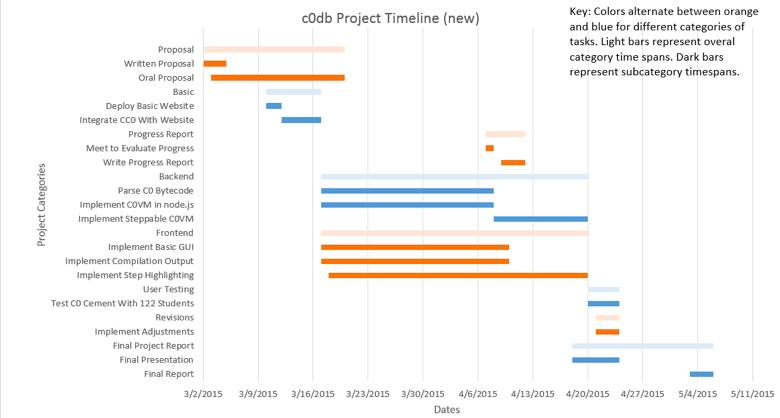
\includegraphics{gannt}

Our revised Gannt chart features two key changes. The back end and front end
sections were modified such that the transition of effort from the virtual
machine to the debugger aligns with where that actually happened. As a result,
the testing and revision section was push back. We are now aiming to start
testing and revision the week of April 20\textsuperscript{th}.

\subsection*{Quantification of Progress}
Currently, we have over 50 test files that we use to check for correctness of
our virtual machine. We currently pass 44 test cases, and are working to have
the rest functioning correctly soon. Once the debugger is more feature complete,
we will focus more on user feedback to assess progress.
